\documentclass[10pt]{article}

\usepackage[margin=0.75in]{geometry}
\usepackage{amsmath,amsthm,amssymb}
\usepackage{xcolor}
\usepackage{cancel}
\usepackage{graphicx}
\usepackage{changepage}
\usepackage{circuitikz}
\usepackage{pgfplots}
\usepackage{physics}
\usepackage{hyperref}
\usepackage{siunitx}
\usepackage{fontspec}
\usepackage{relsize}
\usepackage{subfig}
\usepackage{todonotes}
\usepackage{multicol, multirow, booktabs}
\usepackage[breakable]{tcolorbox}
\usepackage[inline]{enumitem}

\theoremstyle{definition}
\newtheorem{problem}{Problem}
\newtheorem{soln}{Solution}

\pgfplotsset{compat=newest}
\usetikzlibrary{lindenmayersystems}
\usetikzlibrary{arrows}
\usetikzlibrary{calc}
\usetikzlibrary{positioning, fit}
\usetikzlibrary{3d, perspective}

\definecolor{incolor}{HTML}{303F9F}
\definecolor{outcolor}{HTML}{D84315}
\definecolor{cellborder}{HTML}{CFCFCF}
\definecolor{cellbackground}{HTML}{F7F7F7}
\newcommand{\ui}{\hat{i}}
\newcommand{\uj}{\hat{j}}
\newcommand{\uk}{\hat{k}}
\newcommand{\ux}{\hat{x}}
\newcommand{\uy}{\hat{y}}
\newcommand{\uz}{\hat{z}}
\newcommand{\primed}[1]{#1^\prime}
\pgfdeclarelayer{background}  
\pgfsetlayers{background,main}
\AtBeginDocument{\RenewCommandCopy\qty\SI}

\makeatletter
\newcommand{\boxspacing}{\kern\kvtcb@left@rule\kern\kvtcb@boxsep}
\makeatother
\newcommand{\prompt}[4]{
    \ttfamily\llap{{\color{#2}[#3]:\hspace{3pt}#4}}\vspace{-\baselineskip}
}

\newcommand{\thevenin}[2]{
  \begin{center}
    \begin{circuitikz} \draw
      (0,0) -- (2,0) to[battery1, l_=$V_{Th}\eq#1$] (2,2) 
      to[resistor, l_=$R_{Th}\eq#2$] (0,2)
      ;
      \draw [o-] (-.07,2.079);
      \draw [o-] (-.07,0.079);
    \end{circuitikz}
  \end{center}
}

\newcommand{\norton}[2]{
  \begin{center}
    \begin{circuitikz} \draw
      (0,0) -- (3,0) to[american current source, l_=$I_{N}\eq#1$] (3,2) -- (0,2) (2,0)
      to[resistor, l=$R_{N}\eq#2$] (2,2)
      ;
      \draw [o-] (-.07,2.079);
      \draw [o-] (-.07,0.079);
    \end{circuitikz}
  \end{center}
}

\newcommand{\highlight}[1]{\colorbox{yellow}{$\displaystyle #1$}}

\newcommand{\ti}[1]{\widetilde{#1}}

\newfontface{\Kaufmann}{Kaufmann}
\DeclareTextFontCommand{\kf}{\Kaufmann}
\newcommand{\scriptr}{\fontsize{12pt}{12pt}\kf{r}}

\newfontface{\KaufmannB}{Kaufmann Bd BT}
\DeclareTextFontCommand{\kfb}{\KaufmannB}
\newcommand{\bscriptr}{\fontsize{12pt}{12pt}\kfb{r}}

\newcommand{\bv}[1]{\mathbf{#1}}

\title{Physics 3610H: Assignment I}
\author{Jeremy Favro (0805980) \\ Trent University, Peterborough, ON, Canada}
\date{\today}

\begin{document}
\maketitle

% PROBLEM 1
\begin{problem}~
\begin{enumerate}[label=(\alph*)]
  \item Write the value of Euler's number $e$ including 24 digits after the decimal point.
  \item Imagine you took this number, cut it out, and chopped it into 25 pieces such that each
        piece had one digit. Put these pieces in a bag, and choose one at random. What is the
        probability that the number you choose will be a 5?
  \item What is the most probable value
  \item What is the average value
  \item What is the standard deviation
\end{enumerate}
\end{problem}
\begin{soln}~
  \begin{enumerate}[label=(\alph*)]
    \item $e\approx \qty{2.718281828459045235360287}{}$
    \item $n_5/N=3/25=12\%$
    \item ~\\\begin{center}
            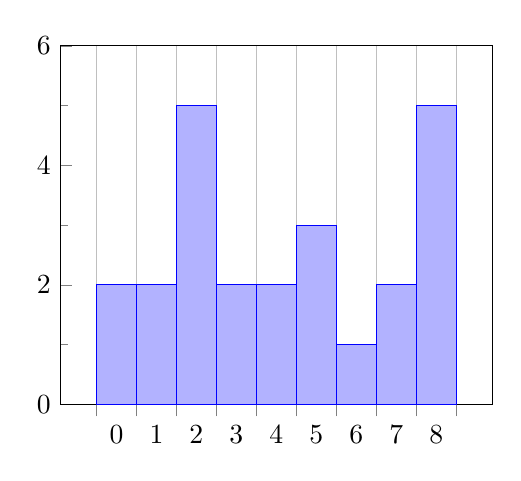
\begin{tikzpicture}
              \begin{axis}[ybar interval, ymax = 6, ymin = 0, minor y tick num = 1, xtick pos = bottom, ytick pos = left, scale=0.8]
                \addplot coordinates { (0, 2) (1, 2) (2, 5) (3, 2) (4, 2) (5, 3) (6, 1) (7, 2) (8, 5) (9, 1)};
              \end{axis}
            \end{tikzpicture}
          \end{center}
          As can be seen by the chart, 8 and 2 are the most probable values in a random draw.
    \item The average is given by
          $$\mu=\frac{1}{N}\sum_{k=0}^{N}kn_i=\frac{1}{25}\left[0\cdot2+1\cdot2+2\cdot 5+ 3\cdot 2 +4\cdot 2 +5\cdot 3 +6\cdot 1 +7\cdot 2 +8\cdot 5 +9\cdot 1\right]=4.4$$
    \item Standard deviation is given by 
          $$\sqrt{\frac{\sum_{k=0}^{N}\left(n_k-\mu\right)^2}{N}}\approx 2.83$$
          (calculated using Python)
  \end{enumerate}
\end{soln}

% PROBLEM 2
\begin{problem}~
\begin{enumerate}[label=(\alph*)]
  \item Consider the complex number $z=3-5i$.
        \begin{enumerate}[label=(\roman*)]
          \item If we express $z$ as $Ae^{i\phi}$, what are $A$ and $\phi$?
          \item What is $z^*$ in both cartesian and polar form?
          \item What is $\left|z\right|^2$
        \end{enumerate}
  \item Consider the function $f(x)=xe^{ix}$
        \begin{enumerate}[label=(\roman*)]
          \item Make a plot of the real part of $f(x)$ as a function of x in the range $(0, 4π)$.
          \item Make a plot of the Imaginary part of $f(x)$ as a function of x in the range $(0, 4π)$.
        \end{enumerate}
\end{enumerate}
\end{problem}
\begin{soln}~
  \begin{enumerate}[label=(\alph*)]
    \item ~
          \begin{enumerate}[label=(\roman*)]
            \item $A=\sqrt{3^2+5^2}=\sqrt{34}$, $\phi=\arctan(-\frac{5}{3})\approx\qty{-1.03}{\radian}$
            \item $z^*=3+5i\approx\sqrt{34}e^{i\qty{1.03}{\radian}}$
            \item $\abs{z}^2=34$
          \end{enumerate}
    \item For ease of plotting, $f(x)=xe^{ix}=x\left(\cos x +i\sin x\right)$ by Euler's formula
          \begin{enumerate}[label=(\roman*)]
            \item ~\\ \begin{center}
                    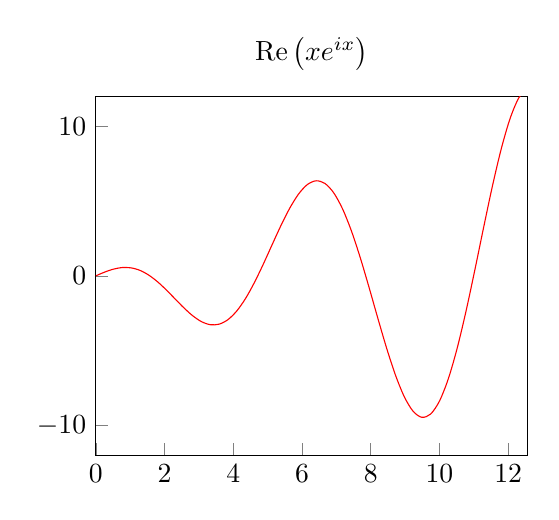
\begin{tikzpicture}
                      \begin{axis}[title = {$\Re \left(xe^{ix}\right)$},
                          ymax = 12,
                          ymin = -12,
                          xmin=0,
                          xmax=4*pi,
                          xtick pos = bottom,
                          ytick pos = left,
                          scale=0.8]
                        \addplot[smooth, domain=0:4*pi, red, samples = 50] {x*cos(deg(x))};
                      \end{axis}
                    \end{tikzpicture}
                  \end{center}
            \item ~\\ \begin{center}
                    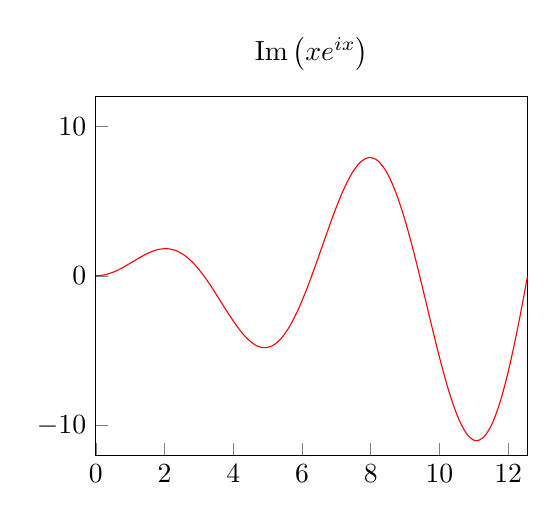
\begin{tikzpicture}
                      \begin{axis}[title = {$\Im \left(xe^{ix}\right)$},
                          ymax = 12,
                          ymin = -12,
                          xmin=0,
                          xmax=4*pi,
                          xtick pos = bottom,
                          ytick pos = left,
                          scale=0.8]
                        \addplot[smooth, domain=0:4*pi, red, samples = 50] {x*sin(deg(x))};
                      \end{axis}
                    \end{tikzpicture}
                  \end{center}
          \end{enumerate}
  \end{enumerate}
\end{soln}
\end{document}